% \documentclass{template/openetcs_article}

% \usepackage{graphicx}

% %\usepackage[top=3cm, bottom=2.5cm, left=3cm, right=2.5cm] {geometry}
% \usepackage {bsymb,b2latex}
% \usepackage{b2latex}
% \usepackage{fancyhdr}
% %\usepackge{lastpage}%
% %\usepackge{color}
% \graphicspath{{./template/}{.}{./images/}}
% %\usepackage[utf8]{inputenc}

%---------------------------------------------------------

\documentclass{template/openetcs_article}
% Use the option "nocc" if the document is not licensed under Creative Commons
%\documentclass[nocc]{template/openetcs_article}
\usepackage {bsymb,b2latex}
\usepackage{lipsum,url,color}
\graphicspath{{./template/}{.}{./images/}}
\begin{document}
\frontmatter
\project{openETCS}

%Please do not change anything above this line
%============================
% The document metadata is defined below

%assign a report number here
\reportnum{OETCS}

%define your workpackage here
\wp{Work-Package 7: ``Toolchain''}


\newcommand{\true}{\ensuremath{true}}
\newcommand{\btext}[1]{{\it #1}}
\newcommand{\bvar}[1]{\btext{#1}}
\newcommand{\bevent}[1]{\btext{#1}}
\newcommand{\binv}[1]{\btext{#1}}
\newcommand{\bconst}[1]{\btext{#1}}
\newcommand{\bparam}[1]{\btext{#1}}
\newcommand{\bfunc}[1]{\btext{#1}}
\newcommand{\baxiom}[1]{\btext{#1}}
\newcommand{\btype}[1]{\btext{#1}}
\newcommand{\bguard}[1]{\btext{#1}}
\newcommand{\bmachine}[1]{\btext{#1}}
\newcommand{\bctx}[1]{\btext{#1}}

\author{Matthias Güdemann\\Systerel, France}

\affiliation{Systerel}

\title{Event-B Model of Subset 026, Section 5.9}

% define the coverart
\coverart[width=350pt]{chart}

\reporttype{Model Description}

%\begin{document}

\maketitle
\tableofcontents
\listoffiguresandtables
\newpage

This document describes a formal model of the requirements of section~5.9 of
the subset 026 of the ETCS specification 3.3.0~\cite{SRS-026-330}. This section
describes the on-sight procedure.

The model is expressed in the formal language Event-B~\cite{abrial-eventB-Book}
and developed within the Rodin tool~\cite{rodin-handbook}. This formalism allows
an iterative modeling approach. In general, one starts with a very abstract
description of the basic functionality and step-wise adds additional details
until the desired level of accuracy of the model is reached. Rodin provides the
necessary proof support to ensure the correctness of the refined behavior.

In this document we present an Event-B model of the procedure on-sight. We use
the iUML plugin which allows for modeling in UML state-charts to create a
graphical model of the procedure which is as close as possible as its
description as flowchart in the section 5.9. The state machine is iteratively
developed using the refinement feature of Event-B. At each refinement step, we
present the reasoning for the step, together with newly introduced variables and
events.

\begin{table}[ht]
  \centering
  \begin{tabular}[ht]{|l|l|}
    \hline
    \hline
  \end{tabular}
  \caption{Glossary}
  \label{tab:glossary}
\end{table}

\section{Short Introduction to Event-B}
\label{sec:short-intr-event}

The formal language Event-B is based on a set-theoretic approach. It is a
variant of the B language, with a focus on system level
modeling~\cite{abrial-eventB-Book}. An Event-B model is separated into a static
and a dynamic part.

The dynamic part of an Event-B model describes abstract state machines. The
state is represented by a set of state variables. A transition from one state to
another is represented by parametrized events which assign new values to the
state variables. Event-B allows unbounded state spaces. They are constrained by
invariants expressed in first order logic with equality which must be fulfilled
in any case. The initial state is created by a special initialization event.

The static part of an Event-B model is represented by contexts. These consist of
carrier sets, constants and axioms. The type system of a model is described by
means of carrier sets and constraints expressed by axioms.

Event-B is not only comprised of descriptions of abstract state machines and
contexts, but also includes a development approach. This approach consists of
iterative refinement of the machines until the desired level of detail is
reached. In the Rodin tool, proof obligations are automatically created which
ensure correct refinement.

Together with the machine invariants, the proof obligations for the refinement
are formally proven, creating proof trees. To accomplish this, there are
different options: many proof obligations can be discharged by automated provers
(e.g., AtelierB, NewPP, Rodin's SMT-plugin), but as the underlying logic is in
general undecidable, it is sometimes necessary to use the interactive proof
support of Rodin.

Any external actions, e.g., mode changes by the driver or train level changes
are modeled via parametrized events. Only events can modify the variables of a
machine. An Event-B model is on the system level, events are assumed to be
called from a software system into which the functional model is embedded. The
guards of the events assure that any event can only be called when appropriate.

\section{Modeling Strategy}
\label{sec:modeling-strategy}

The section~5.9 of the SRS describes the procedure on-sight, in particular it
describes the sequence of mode changes, necessary driver acknowledge and train
brake to enter OS mode, dependent on the current train mode.

For better understanding and to automate many tasks for state based modeling, we
use the iUML plugin~\cite{UML-plugin} which automatically generates Event-B code
representing a state machine specification.

\section{Model Overview}
\label{sec:model-overview}

Figure~\ref{fig:model-overview} shows the structure of the Event-B model. The
left column represents the abstract state machines, the right column the
contexts. An arrow from one machine to another machine represents a refinement
relation, an arrow from a machine to a context represents a sees relation and
arrow from one context to another represents an extension relation.

\begin{figure}[ht]
  \centering
  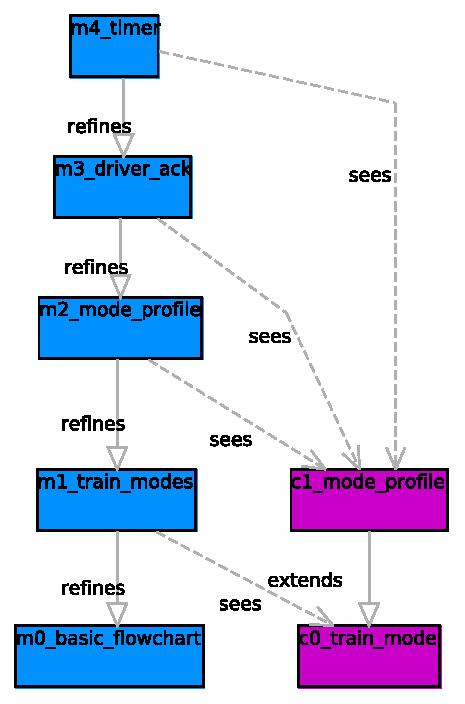
\includegraphics[width=.3\textwidth]{SubSet_026_5_9}
  \caption{Overview on State Machine and Context Hierarchy}
  \label{fig:model-overview}
\end{figure}

The modeling starts with the very abstract possibility to establish and to
terminate a communication session in the machine \bmachine{m0}, the set of
entities is defined in the context \bctx{c0}. This basic functionality is
refined in the succeeding machines to incorporate a more detailed description of
the flowchart.

\section{Model Benefits}
\label{sec:model-highlights}

The Event-B model in Rodin has some interesting properties which are highlighted
here. Some stem from the fact that Rodin is well integrated into the Eclipse
platform which renders many useful plugins available, both those explicitly
developed for integration with Rodin, but also other without Rodin in mind.
Other interesting properties stem from the fact that Rodin and Event-B provide
an extensive proof support for properties.

\begin{itemize}
\item {\bf Graphical Modeling} Through the iUML plugin, Rodin supports graphical
  modeling of UML/SysML state machines. Transitions are labeled with events and
  a fully automatic transformation~\cite{said2009language} creates an Event-B
  representation of the state machine models.
\item {\bf Refinement} In addition to the general refinement which is possible
  in the Event-B approach, the graphical modeling allows to refine the graphical
  state chart models too. For each refinement step, the new details are
  graphically emphasized.
\item {\bf Model Animation} Through the ProB plugin, the graphical models can be
  animated just as textual Event-B models. In this case active transitions can
  be highlighted which helps understand model behavior.
\item {\bf Safety Properties} Using Rodin's proof support and the formalization
  as invariants, it is possible to formalize and prove the identified safety
  properties of the case study (see Section~\ref{sec:machine-3-accepting}).
\end{itemize}

\section{Detailed Model Description}
\label{sec:deta-model-descr}

This section describes in more detail the formal model, beginning from the most
abstract Event-B machine.  For each refinement, the state machine will be shown
and in general only the important manual changes in the model generated from the
state machine. The full generated code and the manual changes are available as a
Rodin project. At each step the additional modeled functionality and its
representation will be described. In particular the initialization event is not
shown for the refined machines. If not mentioned explicitly, sets are
initialized empty, integers with value 0 and Boolean variables with false.

\begin{figure}[ht]
  \centering
  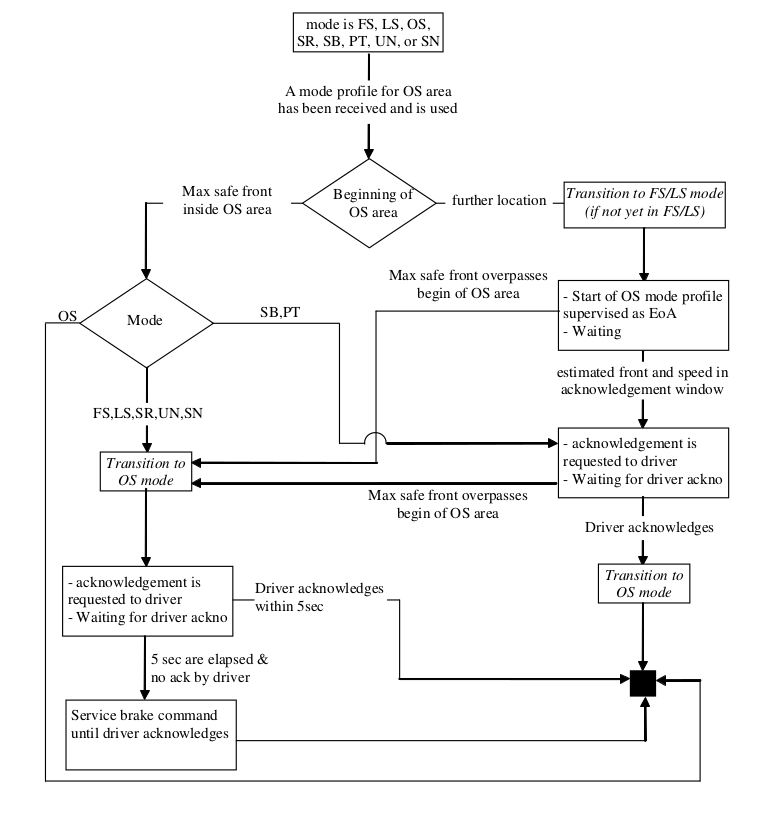
\includegraphics[width=.75\textwidth]{FlowChart}
  \caption{Flowchart for "On-Sight" Procedure~\cite{SRS-026-330}}
  \label{fig:flowchart-OS-mode}
\end{figure}

\subsection{Machine 0 - Basic Flowchart}
\label{sec:machine-0-basic}

The first state machine \bmachine{m0} (see Fig.~\ref{fig:basic-flowchart})
represents an abstract view of the flowchart describing the on-sight procedure
which is shown in §5.9.7 of the SRS~\cite{SRS-026-330} (see
Fig.~\ref{fig:flowchart-OS-mode}).

\begin{figure}[ht]
  \centering
  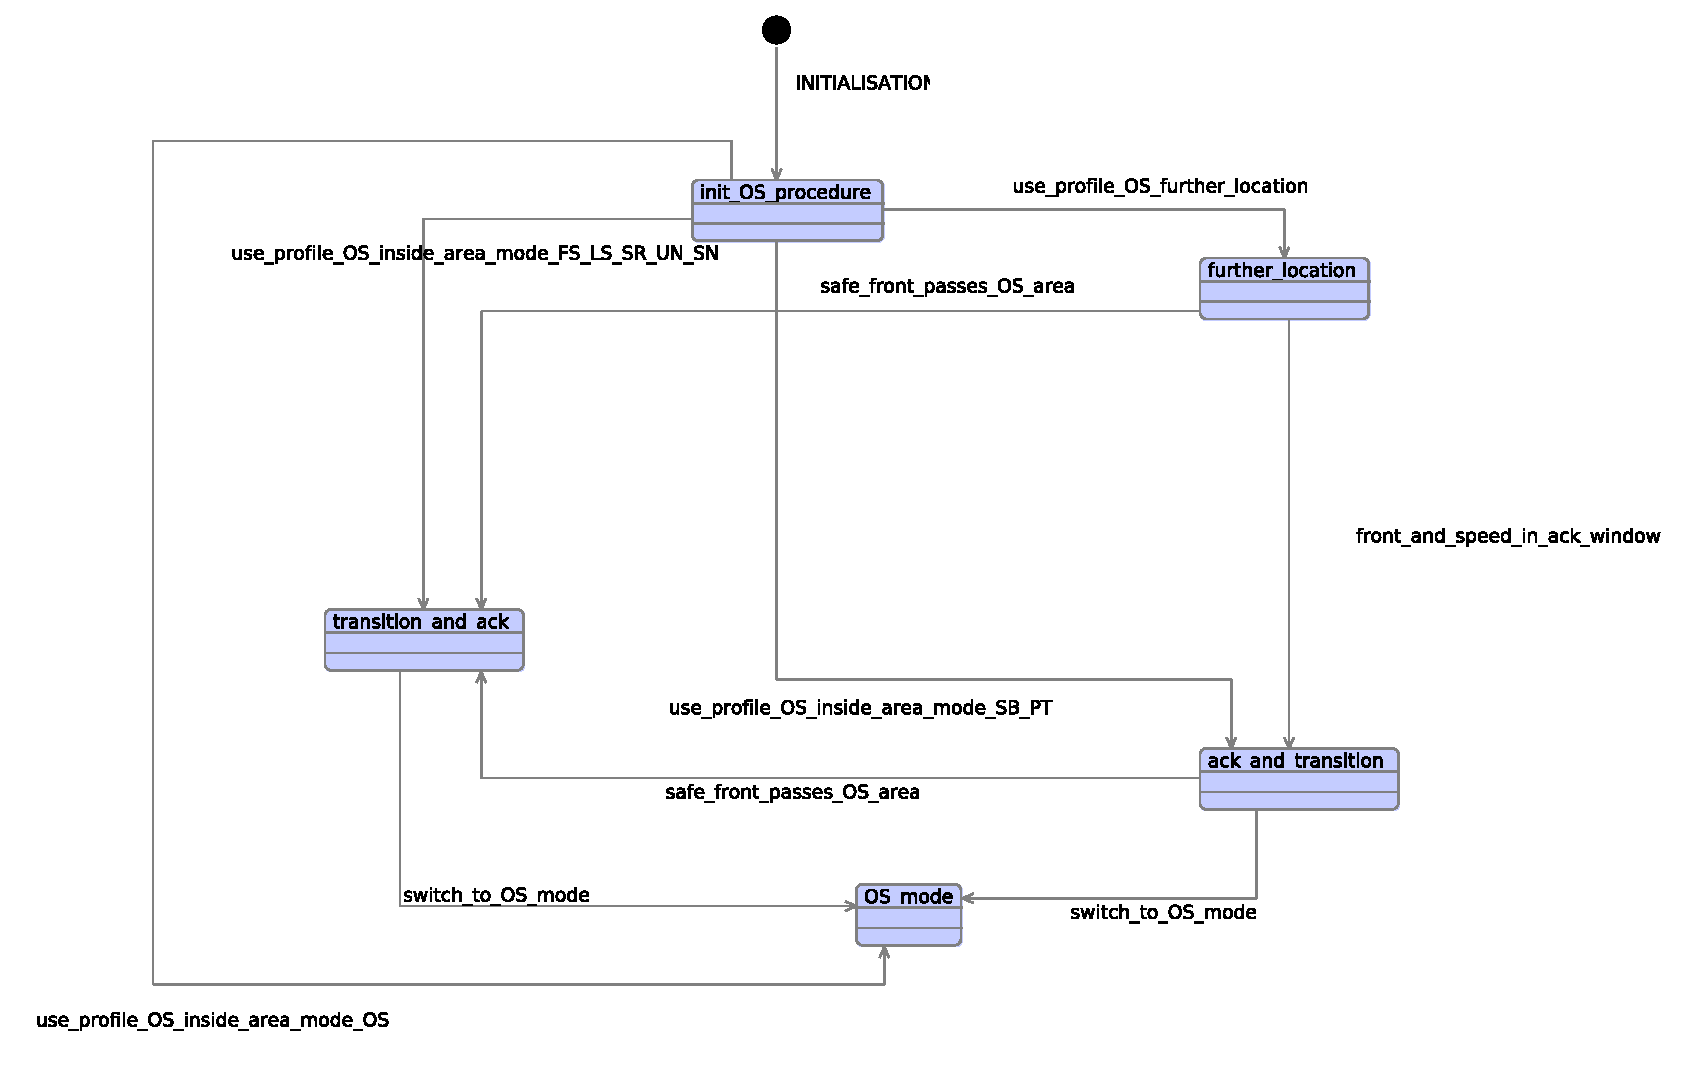
\includegraphics[width=.95\textwidth]{m0_basic_flowchart_on_sight_procedure}
  \caption{Basic Flowchart Representation}
  \label{fig:basic-flowchart}
\end{figure}

The flowchart is translated into a iUML state machine as follows: the initial
state represents the initial situation of the procedure flowchart. The diamonds
of the flowchart represent different cases and are therefore into transitions
with different target states in the state chart. The nodes of the flowchart are
combined for abstraction by combining nodes with multiple incoming flows (or an
initial node) with direct successor nodes.

For example the state \bvar{ack\_and\_transition} can be reached from the
initial state via the event
\bevent{use\_profile\_OS\_inside\_area\_mode\_SB\_PT} and corresponds to the two
lower right nodes of the flowchart. This is justified, as the flow passes two
diamonds in the flowchart, verifying that the i) max safe front of the train is
inside the OS area and ii) the train mode is \bconst{BS} or \bconst{PT}. The
complete model is automatically generated from this state machine. Note
however, that in this abstraction level, there is no concrete notion of train
modes, these appear in the first refinement.

The transitions \bvar{switch\_to\_OS\_mode} signal the completion of the
on-sight procedure, the internal switch to OS mode in the train happens
elsewhere. The state \bvar{OS\_mode} signals the final state.

\subsection{Context 0 - Train Modes}
\label{sec:context-0-entities}

The first context \bvar{c0} specifies the possible modes of the train, these are
of type \btype{t\_train\_modes}. There is one Event-B constant for each possible
mode. The constant \bconst{c\_initial\_mode} represents the initial mode of the
train when the procedure on-sight is started. The constant
\bconst{c\_supervision\_mode} is one mode from the supervision modes.

{\footnotesize
\begin{description}
\SETS
	\begin{description}
		\Item{ t\_train\_modes }
	\end{description}
\CONSTANTS
	\begin{description}
		\ItemY{ c\_FS }{full supervision}
		\ItemY{ c\_LS }{limited supervision}
		\ItemY{ c\_OS }{on sight}
		\ItemY{ c\_SR }{staff responsible}
		\ItemY{ c\_SB }{stand-by}
		\ItemY{ c\_PT }{post-trip}
		\ItemY{ c\_UN }{unfitted}
		\ItemY{ c\_SN }{national system}
		\Item{ c\_initial\_mode }
		\Item{ c\_supervision\_mode }
	\end{description}
\AXIOMS
	\begin{description}
		\nItem{ axm1 }{ partition(t\_train\_modes,\{ c\_FS\} ,\{ c\_LS\} ,\{ c\_OS\} ,\{ c\_SR\} ,		\\\hspace*{6 cm}  \{ c\_SB\} ,\{ c\_PT\} ,\{ c\_UN\} ,\{ c\_SN\} ) }		\nItem{ axm2 }{ c\_initial\_mode \in  \{ c\_FS, c\_OS, c\_PT\}  }		\nItem{ axm3 }{ c\_supervision\_mode \in  \{ c\_LS, c\_FS\}  }	\end{description}
\END
\end{description}

}

\subsection{Machine 1 - Train Modes}
\label{sec:machine-1-train}

The first machine refinement adds the variable \bvar{current\_mode} which tracks
the current mode of the train. This variable is initialized with the value of
\bconst{c\_initial\_mode}.

The state of this variable is used to constrain the guards of the events that
depend on the train modes, i.e., corresponding to those that lead from the
``Mode'' diamond in the flowchart (see Fig.~\ref{fig:flowchart-OS-mode}).
Its state is changed in the \bevent{transition\_to\_supervision\_mode} event
which assigns the value of \bconst{c\_supervision\_mode} or in the
\bevent{transition\_to\_OS\_mode} event which assigns the on-sight mode.

\begin{figure}[ht]
  \centering
  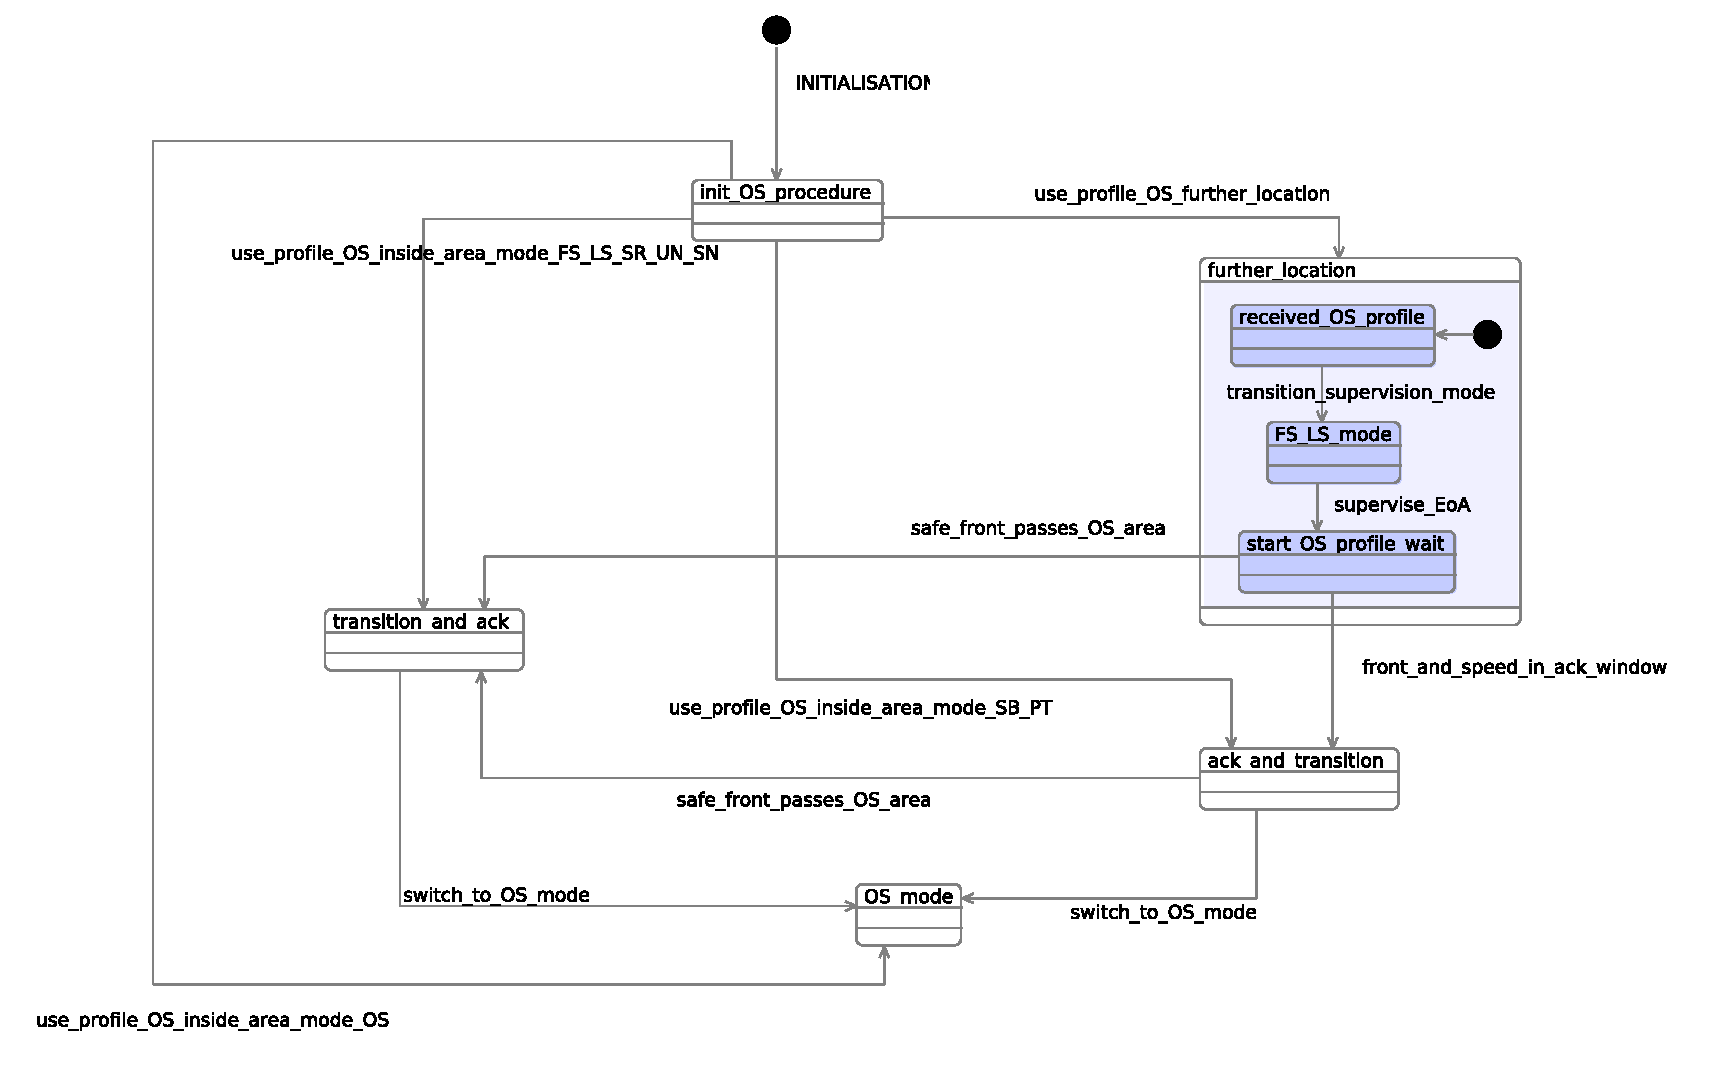
\includegraphics[width=.95\textwidth]{m1_train_modes_on_sight_procedure}
  \caption{First Refinement with Train Modes}
  \label{fig:first-refinement}
\end{figure}

The refined state chart is shown in Fig.~\ref{fig:first-refinement}. The state
\bvar{further\_location} is refined to contain three sub-states and two
events. This switches the train to supervision mode, and starts EoA
supervision. The train stays in this state until either the maximal safe front
passes the OS area or the estimated front and speed leave the acknowledge
window. The exiting transitions are changed to originate from the
\bvar{start\_OS\_profile\_wait} state instead of its super-state. This is
possible as the sub-states correctly refine the super-state.

{\footnotesize
\begin{description}
\MACHINE{m1\_train\_modes}
\REFINES{m0\_basic\_flowchart}
\SEES{c0\_train\_mode}
\VARIABLES
        \begin{description}
                \Item{ current\_mode }
        \end{description}
\INVARIANTS
        \begin{description}
                \nItemY{ inv1 }{ current\_mode \in  t\_train\_modes }{  }
        \end{description}
\EVENTS
        \EVT {safe\_front\_passes\_OS\_area}
        \EXTD {safe\_front\_passes\_OS\_area}
                \begin{description}
                \WhenGrd
                        \begin{description}
                        \nItemX{ isin\_ack\_and\_transition\_or\_isin\_further\_location }{ ack\_and\_transition = TRUE \lor  further\_location = TRUE }
                        \nItem{ isin\_start\_OS\_profile\_wait }{ start\_OS\_profile\_wait = TRUE }
                        \end{description}
                \ThenAct
                        \begin{description}
                        \nItemX{ enter\_transition\_and\_ack }{ transition\_and\_ack :=  TRUE }
                        \nItemX{ leave\_ack\_and\_transition }{ ack\_and\_transition :=  FALSE }
                        \nItemX{ leave\_further\_location }{ further\_location :=  FALSE }
                        \nItem{ leave\_start\_OS\_profile\_wait }{ start\_OS\_profile\_wait :=  FALSE }
                        \end{description}
                \EndAct
                \end{description}
        \EVT {switch\_to\_OS\_mode}
        \EXTD {switch\_to\_OS\_mode}
                \begin{description}
                \WhenGrd
                        \begin{description}
                        \nItemX{ isin\_ack\_and\_transition\_or\_isin\_transition\_and\_ack }{ ack\_and\_transition = TRUE \lor  transition\_and\_ack = TRUE }
                        \end{description}
                \ThenAct
                        \begin{description}
                        \nItemX{ leave\_ack\_and\_transition }{ ack\_and\_transition :=  FALSE }
                        \nItemX{ enter\_OS\_mode }{ OS\_mode :=  TRUE }
                        \nItemX{ leave\_transition\_and\_ack }{ transition\_and\_ack :=  FALSE }
                        \end{description}
                \EndAct
                \end{description}
        \EVT {front\_and\_speed\_in\_ack\_window}
        \EXTD {front\_and\_speed\_in\_ack\_window}
                \begin{description}
                \WhenGrd
                        \begin{description}
                        \nItemX{ isin\_further\_location }{ further\_location = TRUE }
                        \nItem{ isin\_start\_OS\_profile\_wait }{ start\_OS\_profile\_wait = TRUE }
                        \end{description}
                \ThenAct
                        \begin{description}
                        \nItemX{ enter\_ack\_and\_transition }{ ack\_and\_transition :=  TRUE }
                        \nItemX{ leave\_further\_location }{ further\_location :=  FALSE }
                        \nItem{ leave\_start\_OS\_profile\_wait }{ start\_OS\_profile\_wait :=  FALSE }
                        \end{description}
                \EndAct
                \end{description}
        \EVT {use\_profile\_OS\_further\_location}
        \EXTD {use\_profile\_OS\_further\_location}
                \begin{description}
                \WhenGrd
                        \begin{description}
                        \nItemX{ isin\_init\_OS\_procedure }{ init\_OS\_procedure = TRUE }
                        \end{description}
                \ThenAct
                        \begin{description}
                        \nItemX{ leave\_init\_OS\_procedure }{ init\_OS\_procedure :=  FALSE }
                        \nItemX{ enter\_further\_location }{ further\_location :=  TRUE }
                        \nItem{ enter\_received\_OS\_profile }{ received\_OS\_profile :=  TRUE }
                        \end{description}
                \EndAct
                \end{description}
        \EVT {use\_profile\_OS\_inside\_area\_mode\_OS}
        \EXTD {use\_profile\_OS\_inside\_area\_mode\_OS}
                \begin{description}
                \WhenGrd
                        \begin{description}
                        \nItemX{ isin\_init\_OS\_procedure }{ init\_OS\_procedure = TRUE }
                        \nItem{ grd1 }{ current\_mode = c\_OS }
                        \end{description}
                \ThenAct
                        \begin{description}
                        \nItemX{ enter\_OS\_mode }{ OS\_mode :=  TRUE }
                        \nItemX{ leave\_init\_OS\_procedure }{ init\_OS\_procedure :=  FALSE }
                        \end{description}
                \EndAct
                \end{description}
        \EVT {use\_profile\_OS\_inside\_area\_mode\_SB\_PT}
        \EXTD {use\_profile\_OS\_inside\_area\_mode\_SB\_PT}
                \begin{description}
                \WhenGrd
                        \begin{description}
                        \nItemX{ isin\_init\_OS\_procedure }{ init\_OS\_procedure = TRUE }
                        \nItem{ grd1 }{ current\_mode \in  \{ c\_SB, c\_PT\}  }
                        \end{description}
                \ThenAct
                        \begin{description}
                        \nItemX{ enter\_ack\_and\_transition }{ ack\_and\_transition :=  TRUE }
                        \nItemX{ leave\_init\_OS\_procedure }{ init\_OS\_procedure :=  FALSE }
                        \end{description}
                \EndAct
                \end{description}
        \EVT {use\_profile\_OS\_inside\_area\_mode\_FS\_LS\_SR\_UN\_SN}
        \EXTD {use\_profile\_OS\_inside\_area\_mode\_FS\_LS\_SR\_UN\_SN}
                \begin{description}
                \WhenGrd
                        \begin{description}
                        \nItemX{ isin\_init\_OS\_procedure }{ init\_OS\_procedure = TRUE }
                        \nItem{ grd1 }{ current\_mode \in  \{ c\_FS, c\_LS, c\_SR, c\_UN, c\_SN\}  }
                        \end{description}
                \ThenAct
                        \begin{description}
                        \nItemX{ leave\_init\_OS\_procedure }{ init\_OS\_procedure :=  FALSE }
                        \nItemX{ enter\_transition\_and\_ack }{ transition\_and\_ack :=  TRUE }
                        \end{description}
                \EndAct
                \end{description}
        \EVT {transition\_supervision\_mode}
                \begin{description}
                \WhenGrd
                        \begin{description}
                        \nItem{ isin\_received\_OS\_profile }{ received\_OS\_profile = TRUE }
                        \end{description}
                \ThenAct
                        \begin{description}
                        \nItem{ leave\_received\_OS\_profile }{ received\_OS\_profile :=  FALSE }
                        \nItem{ act1 }{ current\_mode :=  c\_supervision\_mode }
                        \nItem{ enter\_FS\_LS\_mode }{ FS\_LS\_mode :=  TRUE }
                        \end{description}
                \EndAct
                \end{description}
        \EVT {transition\_to\_OS\_mode}
                \begin{description}
                \BeginAct
                        \begin{description}
                        \nItem{ act1 }{ current\_mode :=  c\_OS }
                        \end{description}
                \EndAct
                \end{description}
\END
\end{description}

}

\subsection{Context 1 - Mode Profiles}
\label{sec:context-1-mode}

This context extension introduces the type \btype{t\_mode\_profile} for mode
profiles, \btype{t\_train\_fronts} for train fronts (e.g., max safe front,
estimated front), \btype{t\_speed} for train speed and \btype{t\_locations} for
on track locations.

The context also defines several functions, notably one which signals whether a
mode profile specifies an OS area, one which signals whether a given train front
overpasses the OS area for a specific mode profile, one that signals whether a
train front and train speed are in the acknowledge window for a specific mode
profile, one that signals whether a given train front is in the OS area of a
given mode profile and finally a function that returns the EoA from a given
profile.

{\footnotesize
\begin{description}
\CONTEXT{c1\_mode\_profile}
\EXTENDS{c0\_train\_mode}
\SETS
	\begin{description}
		\Item{ t\_mode\_profile }
		\Item{ t\_train\_fronts }
		\Item{ t\_speed }
		\Item{ t\_locations }
	\end{description}
\CONSTANTS
	\begin{description}
		\ItemY{ f\_mode\_profile\_OS\_mode }{indicates whether mode profile demands OS mode}
		\Item{ f\_safe\_train\_front\_overpasses }
		\Item{ f\_estimated\_train\_front\_speed\_in\_window }
		\Item{ c\_profile0 }
		\Item{ f\_safe\_front\_in\_OS\_area }
		\Item{ f\_EoA\_from\_profile }
		\ItemY{ c\_loc0 }{}
		\ItemY{ c\_front0 }{}
	\end{description}
\AXIOMS
	\begin{description}
		\nItem{ axm1 }{ f\_mode\_profile\_OS\_mode \in  t\_mode\_profile \tfun  BOOL }		\nItem{ axm2 }{ f\_safe\_train\_front\_overpasses \in  t\_train\_fronts \cprod  t\_mode\_profile \tfun  BOOL }\cmt{		\\\hspace*{1,4 cm}  train front overpasses begin OS area }
		\nItem{ axm3 }{ f\_estimated\_train\_front\_speed\_in\_window \in  t\_train\_fronts \cprod  t\_mode\_profile \cprod  t\_speed \tfun  BOOL }\cmt{		\\\hspace*{1,4 cm}  est. train front and speed in ack window }
		\nItem{ axm4 }{ c\_profile0 \in  t\_mode\_profile }		\nItem{ axm5 }{ f\_safe\_front\_in\_OS\_area \in  t\_train\_fronts \cprod  t\_mode\_profile \tfun  BOOL }		\nItem{ axm6 }{ f\_EoA\_from\_profile \in  t\_mode\_profile \tfun  t\_locations }\cmt{ }
		\nItem{ axm7 }{ c\_loc0 \in  t\_locations }		\nItem{ axm10 }{ c\_front0 \in  t\_train\_fronts }		\nItem{ axm13 }{ \forall front, profile\qdot front \in  t\_train\_fronts \land  profile \in  t\_mode\_profile \limp 		\\\hspace*{1,8 cm}  (f\_safe\_train\_front\_overpasses(front \mapsto  profile) = TRUE \limp 		\\\hspace*{2,2 cm}  (\forall speed\qdot speed \in  t\_speed \limp  f\_estimated\_train\_front\_speed\_in\_window(front \mapsto  profile \mapsto  speed) = FALSE)) }		\nItem{ axm14 }{ \forall front, profile\qdot front \in  t\_train\_fronts \land  profile \in  t\_mode\_profile \limp 		\\\hspace*{1,8 cm}  (f\_safe\_train\_front\_overpasses(front \mapsto  profile) = FALSE \limp 		\\\hspace*{2,2 cm}  (\exists speed\qdot speed \in  t\_speed \limp  f\_estimated\_train\_front\_speed\_in\_window(front \mapsto  profile \mapsto  speed) = TRUE)) }\cmt{ }
		\nItem{ axm15 }{ \forall profile\qdot profile \in  t\_mode\_profile \limp  (\exists front1, front2\qdot front1 \in  t\_train\_fronts \land  front2 \in  t\_train\_fronts \limp 		\\\hspace*{2,2 cm}  (f\_safe\_front\_in\_OS\_area(front1 \mapsto  profile) \neq  f\_safe\_front\_in\_OS\_area(front2 \mapsto  profile))) }\cmt{		\\\hspace*{1,6 cm}  for each profile there are fronts before and inside the OS area }
	\end{description}
\END

}

\subsection{Machine 2 - Mode Profiles}
\label{sec:machine-2-mode}

The second refinement of the machine introduces the notion of mode profiles,
train fronts (max safe and estimated) and the end of authority (EoA) location
into the model. These are represented by the variables \bvar{EoA\_loc},
\bvar{mode\_profile\_OS}, \bvar{safe\_train\_front} and
\bvar{estimated\_train\_front}.

The train fronts can be changed by the events \bevent{update\_estimated\_front}
and \bevent{update\_safe\_front}. The current values of the fronts, the current
mode profile and its corresponding EoA are used as parameters for the Boolean
functions that guard the events, e.g., for the event
\bevent{safe\_front\_passes\_OS\_area} or for the event
\bevent{front\_and\_speed\_in\_ack\_window}.

\begin{figure}[ht]
  \centering
  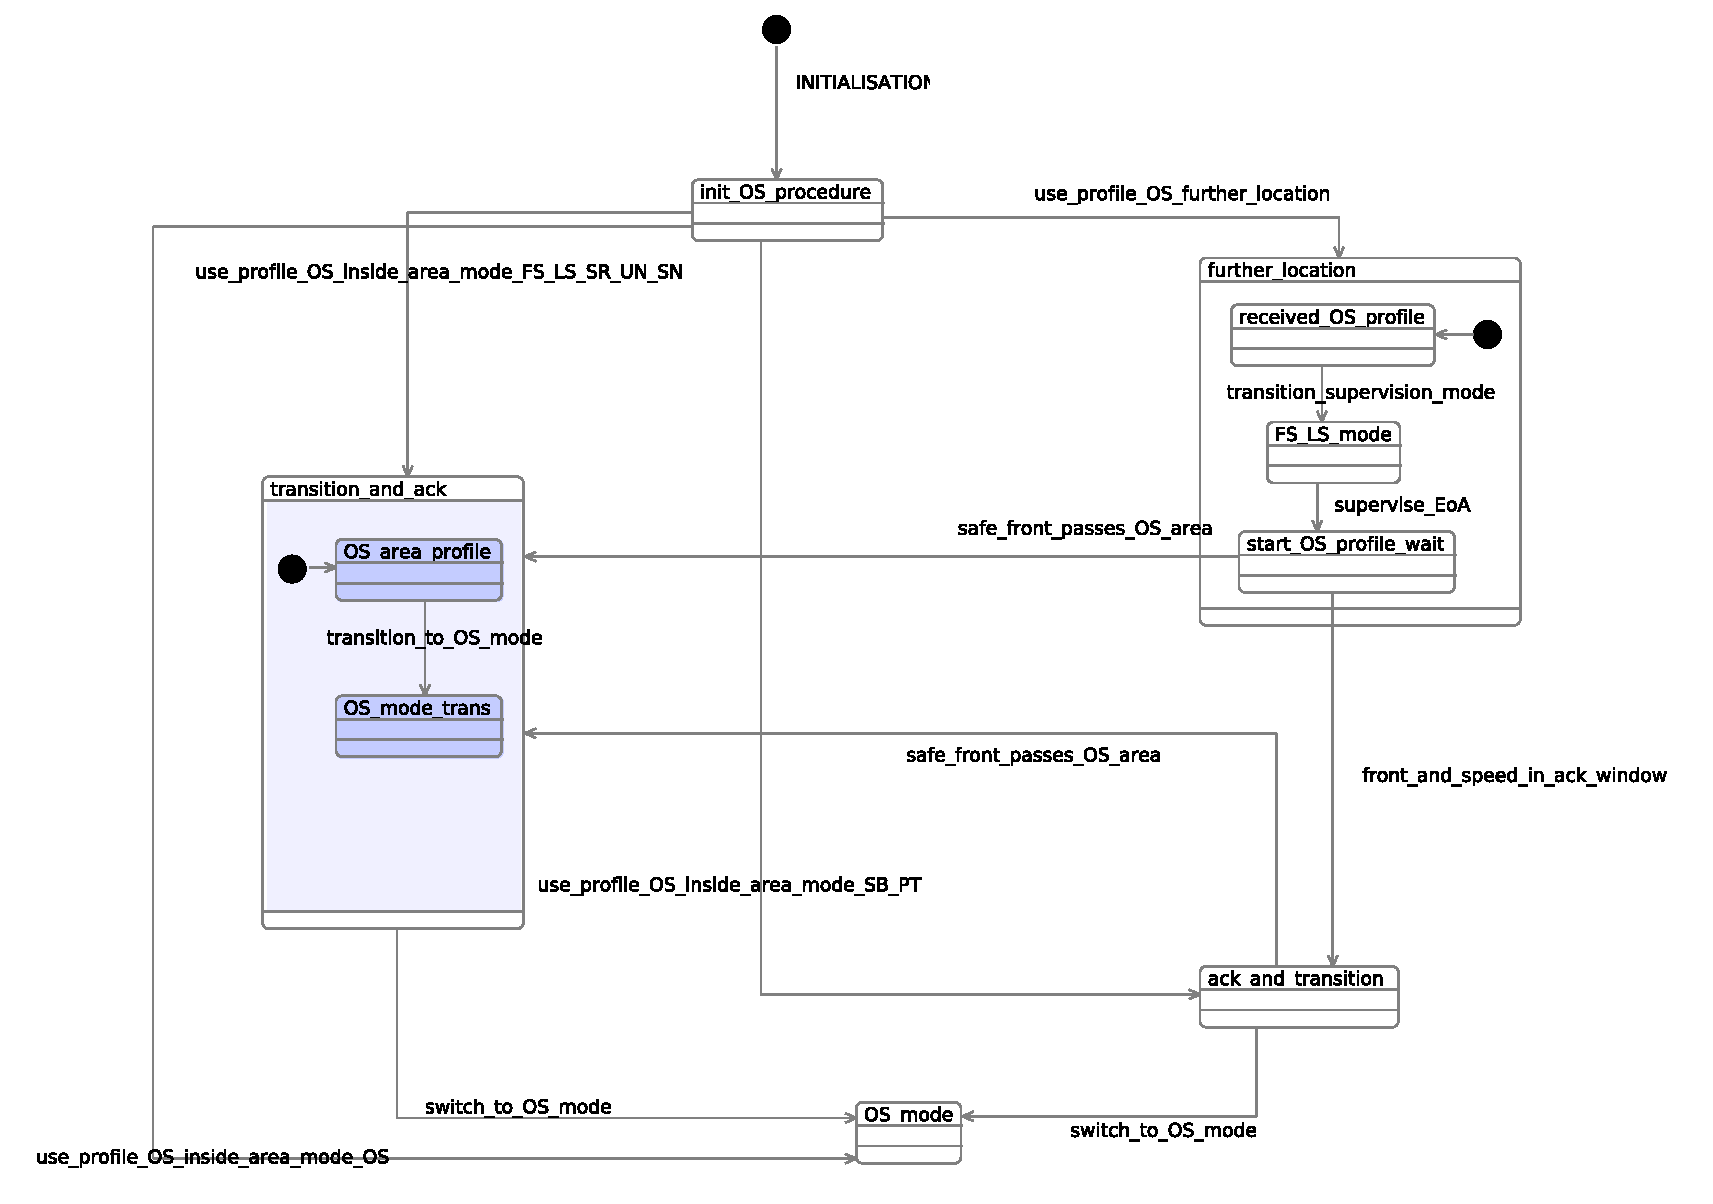
\includegraphics[width=.95\textwidth]{m2_mode_profile_on_sight_procedure}
  \caption{Second Refinement}
  \label{fig:second-refinement}
\end{figure}

The second refinement of the state machine is shown in
Fig.~\ref{fig:second-refinement}. Here the state \bvar{transition\_and\_ack} is
refined with two sub-states. The transition between the two new sub-states
is \bevent{transition\_to\_OS\_mode} which sets the current train mode to
on-sight.

{\footnotesize
\begin{description}
\MACHINE{m2\_mode\_profile}
\REFINES{m1\_train\_modes}
\SEES{c1\_mode\_profile}
\VARIABLES
        \begin{description}
                \ItemY{ EoA\_loc }{}
                \ItemY{ mode\_profile\_OS }{}
                \Item{ safe\_train\_front }
                \Item{ estimated\_train\_front }
        \end{description}
\INVARIANTS
        \begin{description}
                \nItem{ inv1 }{ EoA\_loc \in  t\_locations }
                \nItem{ inv2 }{ mode\_profile\_OS \in  t\_mode\_profile }
                \nItem{ inv3 }{ safe\_train\_front \in  t\_train\_fronts }
                \nItem{ inv4 }{ estimated\_train\_front \in  t\_train\_fronts }
        \end{description}
\EVENTS
        \EVT {safe\_front\_passes\_OS\_area}
        \EXTD {safe\_front\_passes\_OS\_area}
                \begin{description}
                \WhereGrd
                        \begin{description}
                        \nItemX{ isin\_ack\_and\_transition\_or\_isin\_further\_location }{ ack\_and\_transition = TRUE \lor  further\_location = TRUE }
                        \nItemX{ isin\_start\_OS\_profile\_wait }{ start\_OS\_profile\_wait = TRUE }
                        \nItem{ grd1 }{ f\_safe\_train\_front\_overpasses(safe\_train\_front \mapsto  mode\_profile\_OS) = TRUE }
                        \nItemY{ grd2 }{ l\_safe\_train\_front \in  t\_train\_fronts }{ }
                        \end{description}
                \ThenAct
                        \begin{description}
                        \nItemX{ enter\_transition\_and\_ack }{ transition\_and\_ack :=  TRUE }
                        \nItemX{ leave\_ack\_and\_transition }{ ack\_and\_transition :=  FALSE }
                        \nItemX{ leave\_further\_location }{ further\_location :=  FALSE }
                        \nItemX{ leave\_start\_OS\_profile\_wait }{ start\_OS\_profile\_wait :=  FALSE }
                        \nItem{ enter\_OS\_area\_profile }{ OS\_area\_profile :=  TRUE }
                        \end{description}
                \EndAct
                \end{description}
        \EVT {front\_and\_speed\_in\_ack\_window}
        \EXTD {front\_and\_speed\_in\_ack\_window}
                \begin{description}
                \AnyPrm
                        \begin{description}
                        \Item{l\_train\_speed }
                        \end{description}
                \WhereGrd
                        \begin{description}
                        \nItemX{ isin\_further\_location }{ further\_location = TRUE }
                        \nItemX{ isin\_start\_OS\_profile\_wait }{ start\_OS\_profile\_wait = TRUE }
                        \nItem{ grd3 }{ l\_train\_speed \in  t\_speed }
                        \nItem{ grd1 }{ f\_estimated\_train\_front\_speed\_in\_window(estimated\_train\_front \mapsto  mode\_profile\_OS \mapsto  l\_train\_speed) = TRUE }
                        \end{description}
                \ThenAct
                        \begin{description}
                        \nItemX{ enter\_ack\_and\_transition }{ ack\_and\_transition :=  TRUE }
                        \nItemX{ leave\_further\_location }{ further\_location :=  FALSE }
                        \nItemX{ leave\_start\_OS\_profile\_wait }{ start\_OS\_profile\_wait :=  FALSE }
                        \end{description}
                \EndAct
                \end{description}
        \EVT {update\_estimated\_front}
                \begin{description}
                \AnyPrm
                        \begin{description}
                        \Item{l\_front }
                        \end{description}
                \WhereGrd
                        \begin{description}
                        \nItem{ grd1 }{ l\_front \in  t\_train\_fronts }
                        \end{description}
                \ThenAct
                        \begin{description}
                        \nItem{ act1 }{ estimated\_train\_front :=  l\_front }
                        \end{description}
                \EndAct
                \end{description}
        \EVT {update\_safe\_front}
                \begin{description}
                \AnyPrm
                        \begin{description}
                        \ItemY{l\_front }{ }
                        \end{description}
                \WhereGrd
                        \begin{description}
                        \nItem{ grd1 }{ l\_front \in  t\_train\_fronts }
                        \end{description}
                \ThenAct
                        \begin{description}
                        \nItem{ act1 }{ safe\_train\_front :=  l\_front }
                        \end{description}
                \EndAct
                \end{description}
\END
\end{description}

}

\subsection{Machine 3 - Driver Acknowledge}
\label{sec:machine-3-driver}

The third machine refinement introduces the driver acknowledgment. In two cases,
the driver is asked to acknowledge. This is modeled by additional Boolean
variables, two for acknowledging OS mode and two for acknowledging the service
brake. Each time, one variable signals that the driver has been informed that he
has to acknowledge, e.g., for the service brake this is the
\bvar{currently\_asking\_driver\_brake\_ack} variable, and to signal the
completed acknowledge there is the \bconst{driver\_responded\_brake\_ack}
variable. There is also the Boolean variable \bvar{service\_brake} which signals
the active service brake of the train.

\begin{figure}[ht]
  \centering
  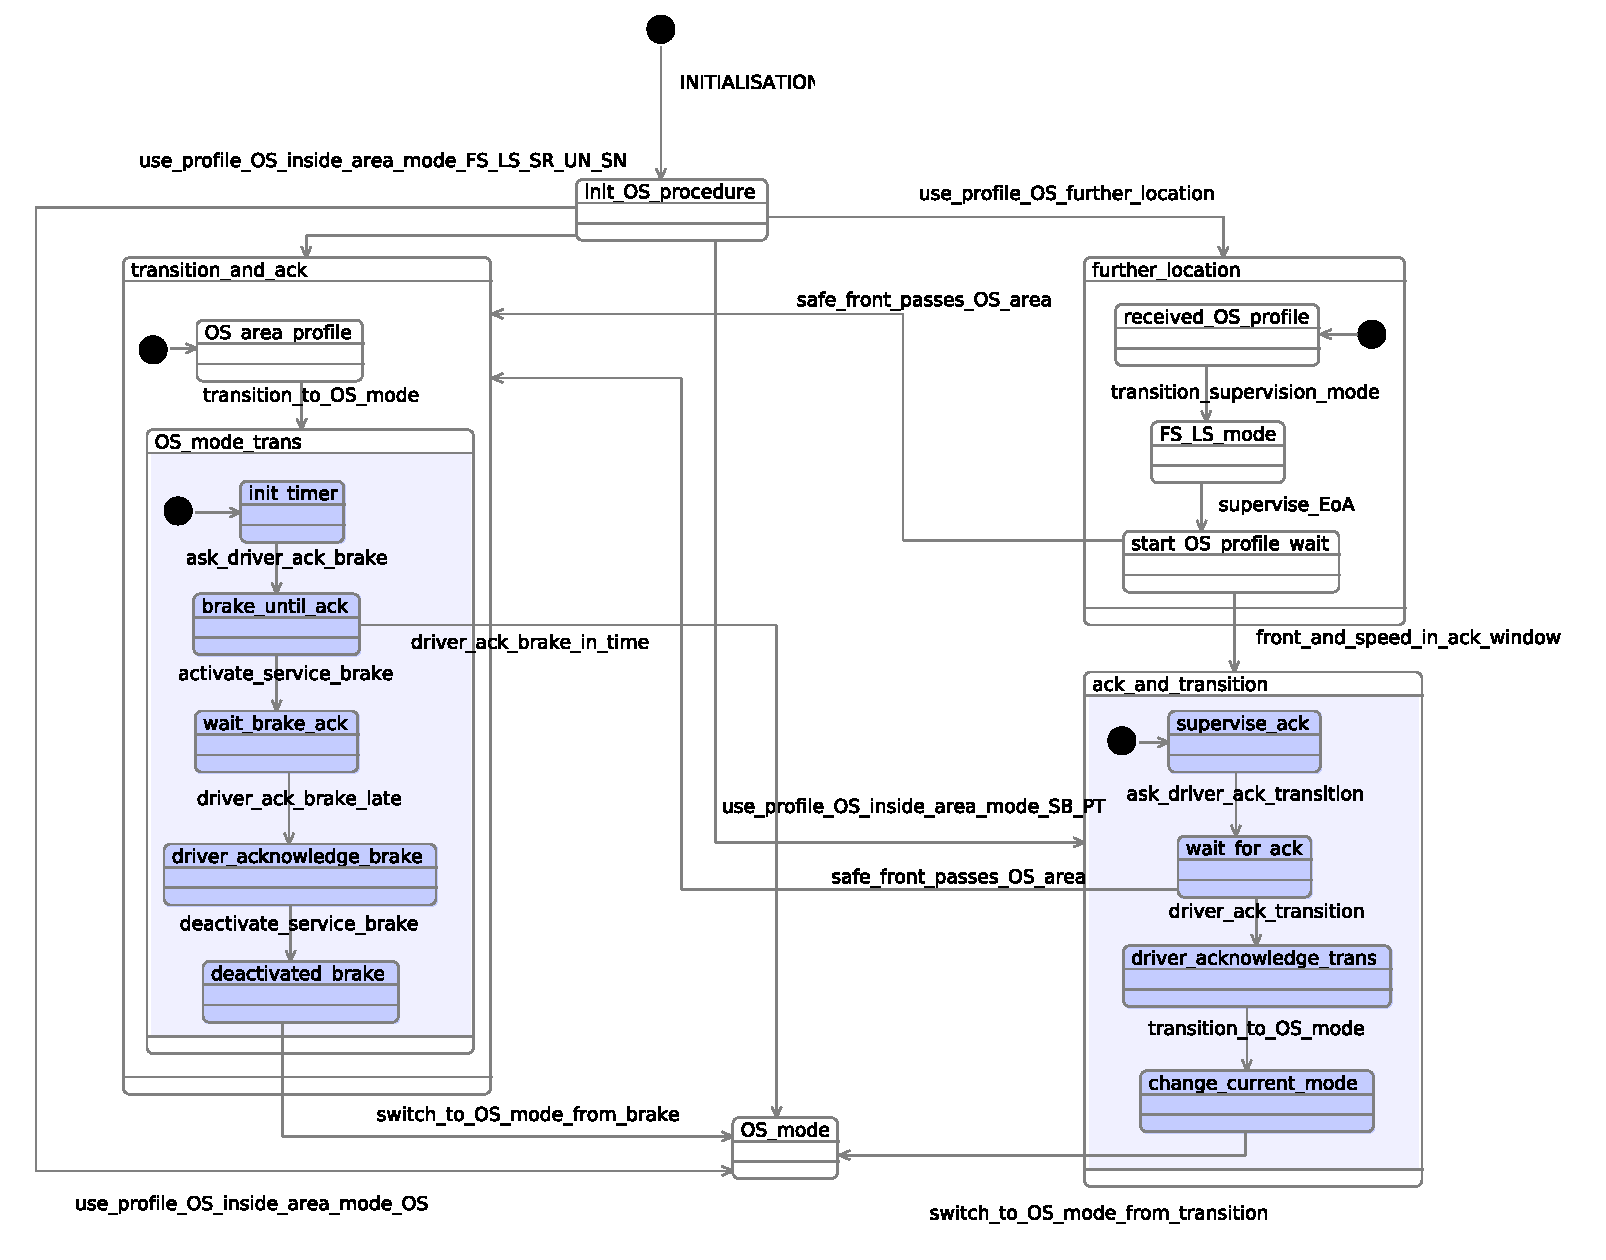
\includegraphics[width=.95\textwidth]{m3_driver_ack_on_sight_procedure}
  \caption{Third Refinement with Driver Acknowledge}
  \label{fig:third-refinement-driver-ack}
\end{figure}

The third refinement of the state machine is shown in
Fig.~\ref{fig:third-refinement-driver-ack}. Here the two states
\bvar{ack\_and\_transition} and \bvar{OS\_mode\_trans} are refined. 

For \bvar{ack\_and\_transition} there are four new sub-states defined. There is
first an event to ask the driver to acknowledge the switch to on-sight mode,
then the OBU waits for the driver acknowledgment. If the max safe train front
passes the OS area without driver acknowledge, then the
\bvar{transition\_and\_ack} state is entered, else the train mode is switched to
on-sight and the final state is entered. Here the outgoing transitions from the
abstract \bvar{ack\_and\_transition} state are change to originate from
\bvar{wait\_for\_ack} or \bvar{change\_current\_mode} respectively. Again this
is possible as the sub-states correctly refine the abstract behavior of the
super state.

The abstract \bvar{OS\_mode\_trans} state is refined by five sub-states. First
the driver is asked to acknowledge the imminent service brake. If he does so in
time, then the procedure finishes and the final state is entered, else the
service brake is activated and stays activated until the driver acknowledges and
the final state is entered.

At this refinement stage, it is possible to prove that whenever the final state
is reached, the mode of the train is on-sight (\binv{inv6}).

{\footnotesize
\begin{description}
\MACHINE{m3\_driver\_ack}
\REFINES{m2\_mode\_profile}
\SEES{c1\_mode\_profile}
\VARIABLES
        \begin{description}
                \Item{ currently\_asking\_driver\_OS\_ack }
                \ItemY{ driver\_responded\_OS\_ack }{}
                \ItemY{ service\_brake\_active }{}
                \ItemY{ currently\_asking\_driver\_brake\_ack }{}
                \Item{ driver\_responded\_brake\_ack }
        \end{description}
\INVARIANTS
        \begin{description}
          \nItemY{ inv6 }{ OS\_mode = TRUE \limp  current\_mode = c\_OS }{}          \end{description}
        \EVENTS
        \EVT {ask\_driver\_ack\_brake}
                \begin{description}
                \WhenGrd
                        \begin{description}
                        \nItem{ isin\_init\_timer }{ init\_timer = TRUE }
                        \nItem{ grd1 }{ currently\_asking\_driver\_brake\_ack = FALSE }
                        \end{description}
                \ThenAct
                        \begin{description}
                        \nItem{ act1 }{ currently\_asking\_driver\_brake\_ack :=  TRUE }
                        \nItem{ enter\_brake\_until\_ack }{ brake\_until\_ack :=  TRUE }
                        \nItem{ act2 }{ driver\_responded\_brake\_ack :=  FALSE }
                        \nItem{ leave\_init\_timer }{ init\_timer :=  FALSE }
                        \end{description}
                \EndAct
                \end{description}
        \EVT {ask\_driver\_ack\_transition}
                \begin{description}
                \WhenGrd
                        \begin{description}
                        \nItem{ isin\_supervise\_ack }{ supervise\_ack = TRUE }
                        \nItem{ grd1 }{ currently\_asking\_driver\_OS\_ack = FALSE }
                        \end{description}
                \ThenAct
                        \begin{description}
                        \nItem{ act1 }{ currently\_asking\_driver\_OS\_ack :=  TRUE }
                        \nItem{ leave\_supervise\_ack }{ supervise\_ack :=  FALSE }
                        \nItem{ enter\_wait\_for\_ack }{ wait\_for\_ack :=  TRUE }
                        \nItem{ act2 }{ driver\_responded\_OS\_ack :=  FALSE }
                        \end{description}
                \EndAct
                \end{description}
        \EVT {driver\_ack\_brake\_in\_time}
        \EXTD {switch\_to\_OS\_mode}
                \begin{description}
                \WhenGrd
                        \begin{description}
                        \nItemX{ isin\_ack\_and\_transition\_or\_isin\_transition\_and\_ack }{ ack\_and\_transition = TRUE \lor  transition\_and\_ack = TRUE }
                        \nItem{ isin\_brake\_until\_ack }{ brake\_until\_ack = TRUE }
                        \nItemY{ grd1 }{ currently\_asking\_driver\_brake\_ack = TRUE }{ }
                        \end{description}
                \ThenAct
                        \begin{description}
                        \nItemX{ leave\_ack\_and\_transition }{ ack\_and\_transition :=  FALSE }
                        \nItemX{ enter\_OS\_mode }{ OS\_mode :=  TRUE }
                        \nItemX{ leave\_transition\_and\_ack }{ transition\_and\_ack :=  FALSE }
                        \nItemX{ leave\_OS\_mode\_trans }{ OS\_mode\_trans :=  FALSE }
                        \nItemX{ leave\_OS\_area\_profile }{ OS\_area\_profile :=  FALSE }
                        \nItem{ act2 }{ driver\_responded\_brake\_ack :=  TRUE }
                        \nItem{ leave\_brake\_until\_ack }{ brake\_until\_ack :=  FALSE }
                        \nItem{ act1 }{ currently\_asking\_driver\_brake\_ack :=  FALSE }
                        \end{description}
                \EndAct
                \end{description}
        \EVT {driver\_ack\_brake\_late}
                \begin{description}
                \WhenGrd
                        \begin{description}
                        \nItem{ grd1 }{ currently\_asking\_driver\_brake\_ack = TRUE }
                        \nItem{ isin\_wait\_brake\_ack }{ wait\_brake\_ack = TRUE }
                        \end{description}
                \ThenAct
                        \begin{description}
                        \nItem{ act1 }{ currently\_asking\_driver\_brake\_ack :=  FALSE }
                        \nItem{ enter\_driver\_acknowledge\_brake }{ driver\_acknowledge\_brake :=  TRUE }
                        \nItem{ act2 }{ driver\_responded\_brake\_ack :=  TRUE }
                        \nItem{ leave\_wait\_brake\_ack }{ wait\_brake\_ack :=  FALSE }
                        \end{description}
                \EndAct
                \end{description}
        \EVT {driver\_ack\_transition}
                \begin{description}
                \WhenGrd
                        \begin{description}
                        \nItem{ grd1 }{ currently\_asking\_driver\_OS\_ack = TRUE }
                        \nItem{ isin\_wait\_for\_ack }{ wait\_for\_ack = TRUE }
                        \end{description}
                \ThenAct
                        \begin{description}
                        \nItem{ act2 }{ driver\_responded\_OS\_ack :=  TRUE }
                        \nItem{ enter\_driver\_acknowledge\_trans }{ driver\_acknowledge\_trans :=  TRUE }
                        \nItem{ leave\_wait\_for\_ack }{ wait\_for\_ack :=  FALSE }
                        \nItem{ act1 }{ currently\_asking\_driver\_OS\_ack :=  FALSE }
                        \end{description}
                \EndAct
                \end{description}
        \EVT {activate\_service\_brake}
                \begin{description}
                \WhenGrd
                        \begin{description}
                        \nItem{ grd1 }{ service\_brake\_active = FALSE }
                        \nItem{ isin\_brake\_until\_ack }{ brake\_until\_ack = TRUE }
                        \end{description}
                \ThenAct
                        \begin{description}
                        \nItem{ act1 }{ service\_brake\_active :=  TRUE }
                        \nItem{ leave\_brake\_until\_ack }{ brake\_until\_ack :=  FALSE }
                        \nItem{ enter\_wait\_brake\_ack }{ wait\_brake\_ack :=  TRUE }
                        \end{description}
                \EndAct
                \end{description}
        \EVT {deactivate\_service\_brake}
                \begin{description}
                \WhenGrd
                        \begin{description}
                        \nItem{ grd1 }{ service\_brake\_active = TRUE }
                        \nItem{ isin\_driver\_acknowledge\_brake }{ driver\_acknowledge\_brake = TRUE }
                        \end{description}
                \ThenAct
                        \begin{description}
                        \nItem{ enter\_deactivated\_brake }{ deactivated\_brake :=  TRUE }
                        \nItemY{ act2 }{ service\_brake\_active :=  FALSE }{  }
                        \nItem{ act3 }{ driver\_responded\_brake\_ack :=  FALSE }
                        \nItem{ leave\_driver\_acknowledge\_brake }{ driver\_acknowledge\_brake :=  FALSE }
                        \end{description}
                \EndAct
                \end{description}
\END
\end{description}

}

\subsection{Machine 4 - Timeout}
\label{sec:machine-4-timeout}


\begin{figure}[ht]
  \centering
  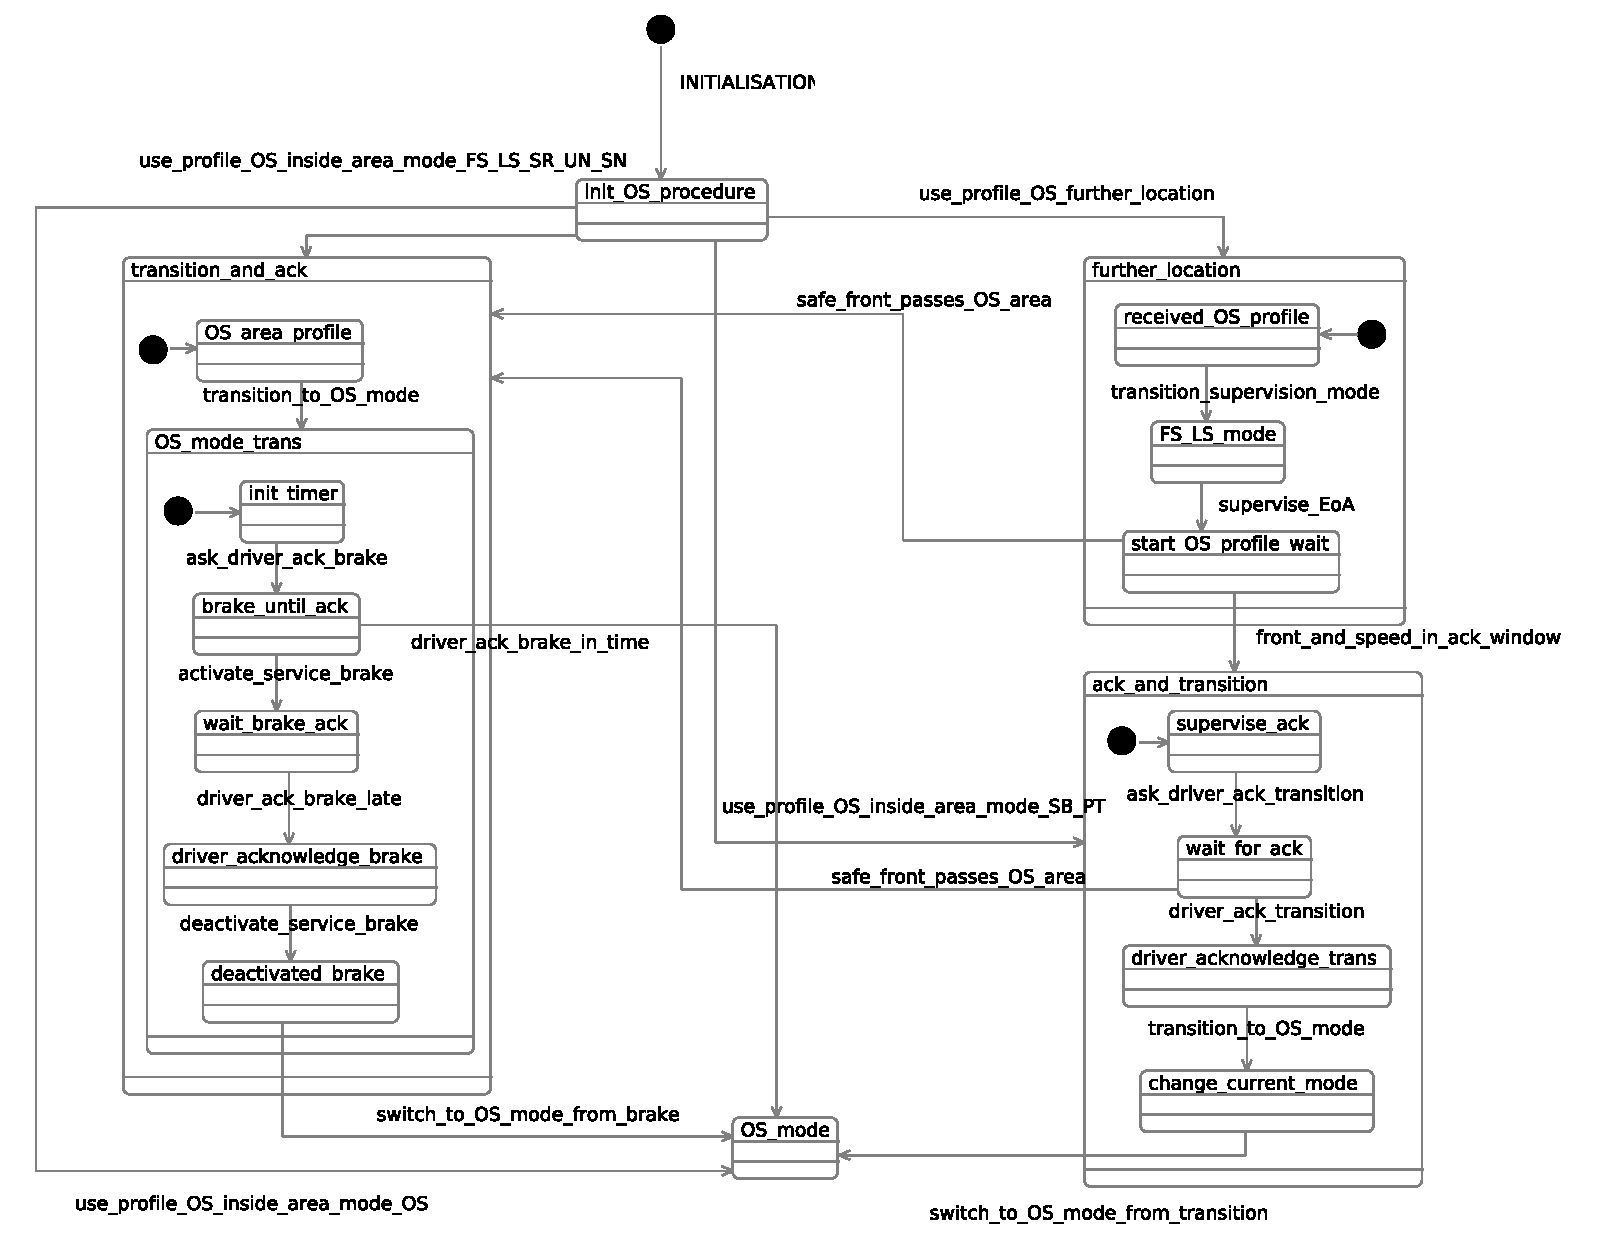
\includegraphics[width=.95\textwidth]{m4_timeout_on_sight_procedure}
  \caption{Fourth Refinement State Machine}
  \label{fig:fourth-refinement-state-machine}
\end{figure}

{\footnotesize
\documentclass[10pt,a4paper]{report}
\usepackage[top=3cm, bottom=2.5cm, left=3cm, right=2.5cm] {geometry}
\usepackage {bsymb,b2latex}
\usepackage[utf8]{inputenc}
\usepackage{fancyhdr,lastpage,color}
\lhead{\rm An Event-B Specification of m4\_timeout}
\rhead {\rm Page \thepage~of \pageref{LastPage}}
\lfoot{}\cfoot{}\rfoot{}
\pagestyle{fancy}
%---------------------------------------------------------
\begin{document}
\thispagestyle{empty}
\begin{description}
\BTitle{m4\_timeout}{8Apr2013}{02:46:18 PM}
\MACHINE{m4\_timeout}
\REFINES{m3\_driver\_ack}
\SEES{c1\_mode\_profile}
\VARIABLES
	\begin{description}
		\Item{ init\_OS\_procedure }
		\Item{ further\_location }
		\Item{ received\_OS\_profile }
		\Item{ FS\_LS\_mode }
		\Item{ start\_OS\_profile\_wait }
		\Item{ ack\_and\_transition }
		\Item{ supervise\_ack }
		\Item{ wait\_for\_ack }
		\Item{ driver\_acknowledge\_trans }
		\Item{ change\_current\_mode }
		\Item{ transition\_and\_ack }
		\Item{ OS\_area\_profile }
		\Item{ OS\_mode\_trans }
		\Item{ init\_timer }
		\Item{ wait\_brake\_ack }
		\Item{ brake\_until\_ack }
		\Item{ driver\_acknowledge\_brake }
		\Item{ deactivated\_brake }
		\Item{ OS\_mode }
		\ItemY{ current\_mode }{}
		\ItemY{ EoA\_loc }{}
		\ItemY{ mode\_profile\_OS }{}
		\Item{ safe\_train\_front }
		\ItemY{ estimated\_train\_front }{}
		\Item{ currently\_asking\_driver\_OS\_ack }
		\ItemY{ driver\_responded\_OS\_ack }{}
		\ItemY{ service\_brake\_active }{}
		\ItemY{ currently\_asking\_driver\_brake\_ack }{}
		\Item{ driver\_responded\_brake\_ack }
		\Item{ timer\_expired }
	\end{description}
\INVARIANTS
	\begin{description}
		\nItemY{ inv1 }{ timer\_expired \in  BOOL }{  }
		\nItem{ inv2 }{  }
	\end{description}
\EVENTS
	\INITIALISATION
		\\\textit{extended}\cmt{ }
		\begin{description}
		\BeginAct
			\begin{description}
			\nItemX{ init\_further\_location }{ further\_location :=  FALSE }
			\nItemX{ init\_transition\_and\_ack }{ transition\_and\_ack :=  FALSE }
			\nItemX{ init\_ack\_and\_transition }{ ack\_and\_transition :=  FALSE }
			\nItemX{ init\_init\_OS\_procedure }{ init\_OS\_procedure :=  TRUE }
			\nItemX{ init\_OS\_mode }{ OS\_mode :=  FALSE }
			\nItemX{ init\_FS\_LS\_mode }{ FS\_LS\_mode :=  FALSE }
			\nItemX{ init\_start\_OS\_profile\_wait }{ start\_OS\_profile\_wait :=  FALSE }
			\nItemX{ act1 }{ current\_mode :=  c\_initial\_mode }
			\nItemX{ init\_received\_OS\_profile }{ received\_OS\_profile :=  FALSE }
			\nItemX{ act2 }{ EoA\_loc :=  c\_loc0 }
			\nItemX{ init\_OS\_area\_profile }{ OS\_area\_profile :=  FALSE }
			\nItemXY{ act3 }{ mode\_profile\_OS :=  c\_profile0 }{  }
			\nItemXY{ init\_OS\_mode\_trans }{ OS\_mode\_trans :=  FALSE }{  }
			\nItemX{ act4 }{ safe\_train\_front :=  c\_front0 }
			\nItemX{ act5 }{ estimated\_train\_front :=  c\_front0 }
			\nItemX{ init\_deactivated\_brake }{ deactivated\_brake :=  FALSE }
			\nItemXY{ act7 }{ driver\_responded\_OS\_ack :=  FALSE }{  }
			\nItemX{ act6 }{ currently\_asking\_driver\_OS\_ack :=  FALSE }
			\nItemX{ act8 }{ service\_brake\_active :=  FALSE }
			\nItemX{ init\_wait\_brake\_ack }{ wait\_brake\_ack :=  FALSE }
			\nItemX{ act9 }{ currently\_asking\_driver\_brake\_ack :=  FALSE }
			\nItemX{ init\_wait\_for\_ack }{ wait\_for\_ack :=  FALSE }
			\nItemX{ init\_supervise\_ack }{ supervise\_ack :=  FALSE }
			\nItemX{ init\_driver\_acknowledge\_trans }{ driver\_acknowledge\_trans :=  FALSE }
			\nItemX{ init\_init\_timer }{ init\_timer :=  FALSE }
			\nItemX{ init\_change\_current\_mode }{ change\_current\_mode :=  FALSE }
			\nItemX{ act10 }{ driver\_responded\_brake\_ack :=  FALSE }
			\nItemX{ init\_driver\_acknowledge\_brake }{ driver\_acknowledge\_brake :=  FALSE }
			\nItemX{ init\_brake\_until\_ack }{ brake\_until\_ack :=  FALSE }
			\nItem{ act11 }{ timer\_expired :=  FALSE }
			\end{description}
		\EndAct
		\end{description}
	\EVT {safe\_front\_passes\_OS\_area}
	\EXTD {safe\_front\_passes\_OS\_area}
		\begin{description}
		\WhenGrd
			\begin{description}
			\nItemX{ isin\_ack\_and\_transition\_or\_isin\_further\_location }{ ack\_and\_transition = TRUE \lor  further\_location = TRUE }
			\nItemX{ isin\_start\_OS\_profile\_wait }{ start\_OS\_profile\_wait = TRUE }
			\nItemX{ grd1 }{ f\_safe\_train\_front\_overpasses(safe\_train\_front \mapsto  mode\_profile\_OS) = TRUE }
			\nItemX{ isin\_wait\_for\_ack }{ wait\_for\_ack = TRUE }
			\end{description}
		\ThenAct
			\begin{description}
			\nItemX{ enter\_transition\_and\_ack }{ transition\_and\_ack :=  TRUE }
			\nItemX{ leave\_ack\_and\_transition }{ ack\_and\_transition :=  FALSE }
			\nItemX{ leave\_further\_location }{ further\_location :=  FALSE }
			\nItemX{ leave\_start\_OS\_profile\_wait }{ start\_OS\_profile\_wait :=  FALSE }
			\nItemX{ enter\_OS\_area\_profile }{ OS\_area\_profile :=  TRUE }
			\nItemX{ leave\_wait\_for\_ack }{ wait\_for\_ack :=  FALSE }
			\end{description}
		\EndAct
		\end{description}
	\EVT {switch\_to\_OS\_mode\_from\_brake}
	\EXTD {switch\_to\_OS\_mode\_from\_brake}
		\begin{description}
		\WhenGrd
			\begin{description}
			\nItemX{ isin\_ack\_and\_transition\_or\_isin\_transition\_and\_ack }{ ack\_and\_transition = TRUE \lor  transition\_and\_ack = TRUE }
			\nItemX{ isin\_deactivated\_brake }{ deactivated\_brake = TRUE }
			\end{description}
		\ThenAct
			\begin{description}
			\nItemX{ leave\_ack\_and\_transition }{ ack\_and\_transition :=  FALSE }
			\nItemX{ enter\_OS\_mode }{ OS\_mode :=  TRUE }
			\nItemX{ leave\_transition\_and\_ack }{ transition\_and\_ack :=  FALSE }
			\nItemX{ leave\_OS\_mode\_trans }{ OS\_mode\_trans :=  FALSE }
			\nItemX{ leave\_OS\_area\_profile }{ OS\_area\_profile :=  FALSE }
			\nItemX{ leave\_deactivated\_brake }{ deactivated\_brake :=  FALSE }
			\end{description}
		\EndAct
		\end{description}
	\EVT {switch\_to\_OS\_mode\_from\_transition}
	\EXTD {switch\_to\_OS\_mode\_from\_transition}
		\begin{description}
		\WhenGrd
			\begin{description}
			\nItemX{ isin\_ack\_and\_transition\_or\_isin\_transition\_and\_ack }{ ack\_and\_transition = TRUE \lor  transition\_and\_ack = TRUE }
			\nItemX{ isin\_change\_current\_mode }{ change\_current\_mode = TRUE }
			\end{description}
		\ThenAct
			\begin{description}
			\nItemX{ leave\_ack\_and\_transition }{ ack\_and\_transition :=  FALSE }
			\nItemX{ enter\_OS\_mode }{ OS\_mode :=  TRUE }
			\nItemX{ leave\_transition\_and\_ack }{ transition\_and\_ack :=  FALSE }
			\nItemX{ leave\_OS\_mode\_trans }{ OS\_mode\_trans :=  FALSE }
			\nItemX{ leave\_OS\_area\_profile }{ OS\_area\_profile :=  FALSE }
			\nItemX{ leave\_change\_current\_mode }{ change\_current\_mode :=  FALSE }
			\end{description}
		\EndAct
		\end{description}
	\EVT {front\_and\_speed\_in\_ack\_window}
	\EXTD {front\_and\_speed\_in\_ack\_window}
		\begin{description}
		\AnyPrm
			\begin{description}
			\ItemX{l\_train\_speed }
			\end{description}
		\WhereGrd
			\begin{description}
			\nItemX{ isin\_further\_location }{ further\_location = TRUE }
			\nItemX{ isin\_start\_OS\_profile\_wait }{ start\_OS\_profile\_wait = TRUE }
			\nItemX{ grd3 }{ l\_train\_speed \in  t\_speed }
			\nItemX{ grd1 }{ f\_estimated\_train\_front\_speed\_in\_window(estimated\_train\_front \mapsto  mode\_profile\_OS \mapsto  l\_train\_speed) = TRUE }
			\end{description}
		\ThenAct
			\begin{description}
			\nItemX{ enter\_ack\_and\_transition }{ ack\_and\_transition :=  TRUE }
			\nItemX{ leave\_further\_location }{ further\_location :=  FALSE }
			\nItemX{ leave\_start\_OS\_profile\_wait }{ start\_OS\_profile\_wait :=  FALSE }
			\nItemX{ enter\_supervise\_ack }{ supervise\_ack :=  TRUE }
			\end{description}
		\EndAct
		\end{description}
	\EVT {use\_profile\_OS\_further\_location}
	\EXTD {use\_profile\_OS\_further\_location}
		\begin{description}
		\WhenGrd
			\begin{description}
			\nItemX{ isin\_init\_OS\_procedure }{ init\_OS\_procedure = TRUE }
			\nItemXY{ grd1 }{ f\_safe\_front\_in\_OS\_area(safe\_train\_front \mapsto  mode\_profile\_OS) = FALSE }{ } 
			\end{description}
		\ThenAct
			\begin{description}
			\nItemX{ leave\_init\_OS\_procedure }{ init\_OS\_procedure :=  FALSE }
			\nItemX{ enter\_further\_location }{ further\_location :=  TRUE }
			\nItemX{ enter\_received\_OS\_profile }{ received\_OS\_profile :=  TRUE }
			\end{description}
		\EndAct
		\end{description}
	\EVT {use\_profile\_OS\_inside\_area\_mode\_OS}
	\EXTD {use\_profile\_OS\_inside\_area\_mode\_OS}
		\begin{description}
		\WhenGrd
			\begin{description}
			\nItemX{ isin\_init\_OS\_procedure }{ init\_OS\_procedure = TRUE }
			\nItemX{ grd1 }{ current\_mode = c\_OS }
			\nItemXY{ grd2 }{ f\_safe\_front\_in\_OS\_area(safe\_train\_front \mapsto  mode\_profile\_OS) = TRUE }{ } 
			\end{description}
		\ThenAct
			\begin{description}
			\nItemX{ enter\_OS\_mode }{ OS\_mode :=  TRUE }
			\nItemX{ leave\_init\_OS\_procedure }{ init\_OS\_procedure :=  FALSE }
			\end{description}
		\EndAct
		\end{description}
	\EVT {use\_profile\_OS\_inside\_area\_mode\_SB\_PT}
	\EXTD {use\_profile\_OS\_inside\_area\_mode\_SB\_PT}
		\begin{description}
		\WhenGrd
			\begin{description}
			\nItemX{ isin\_init\_OS\_procedure }{ init\_OS\_procedure = TRUE }
			\nItemX{ grd1 }{ current\_mode \in  \{ c\_SB, c\_PT\}  }
			\nItemX{ grd2 }{ f\_safe\_front\_in\_OS\_area(safe\_train\_front \mapsto  mode\_profile\_OS) = FALSE }
			\end{description}
		\ThenAct
			\begin{description}
			\nItemX{ enter\_ack\_and\_transition }{ ack\_and\_transition :=  TRUE }
			\nItemX{ leave\_init\_OS\_procedure }{ init\_OS\_procedure :=  FALSE }
			\nItemX{ enter\_supervise\_ack }{ supervise\_ack :=  TRUE }
			\end{description}
		\EndAct
		\end{description}
	\EVT {use\_profile\_OS\_inside\_area\_mode\_FS\_LS\_SR\_UN\_SN}
	\EXTD {use\_profile\_OS\_inside\_area\_mode\_FS\_LS\_SR\_UN\_SN}
		\begin{description}
		\WhenGrd
			\begin{description}
			\nItemX{ isin\_init\_OS\_procedure }{ init\_OS\_procedure = TRUE }
			\nItemX{ grd1 }{ current\_mode \in  \{ c\_FS, c\_LS, c\_SR, c\_UN, c\_SN\}  }
			\nItemXY{ grd2 }{ f\_safe\_front\_in\_OS\_area(safe\_train\_front \mapsto  mode\_profile\_OS) = TRUE }{ } 
			\end{description}
		\ThenAct
			\begin{description}
			\nItemX{ leave\_init\_OS\_procedure }{ init\_OS\_procedure :=  FALSE }
			\nItemX{ enter\_transition\_and\_ack }{ transition\_and\_ack :=  TRUE }
			\nItemX{ enter\_OS\_area\_profile }{ OS\_area\_profile :=  TRUE }
			\end{description}
		\EndAct
		\end{description}
	\EVT {transition\_supervision\_mode}
	\EXTD {transition\_supervision\_mode}
		\begin{description}
		\WhenGrd
			\begin{description}
			\nItemX{ isin\_received\_OS\_profile }{ received\_OS\_profile = TRUE }
			\end{description}
		\ThenAct
			\begin{description}
			\nItemX{ leave\_received\_OS\_profile }{ received\_OS\_profile :=  FALSE }
			\nItemX{ act1 }{ current\_mode :=  c\_supervision\_mode }
			\nItemX{ enter\_FS\_LS\_mode }{ FS\_LS\_mode :=  TRUE }
			\end{description}
		\EndAct
		\end{description}
	\EVT {supervise\_EoA}
	\EXTD {supervise\_EoA}
		\begin{description}
		\WhenGrd
			\begin{description}
			\nItemXY{ isin\_FS\_LS\_mode }{ FS\_LS\_mode = TRUE }{ } 
			\end{description}
		\ThenAct
			\begin{description}
			\nItemX{ leave\_FS\_LS\_mode }{ FS\_LS\_mode :=  FALSE }
			\nItemX{ enter\_start\_OS\_profile\_wait }{ start\_OS\_profile\_wait :=  TRUE }
			\end{description}
		\EndAct
		\end{description}
	\EVT {transition\_to\_OS\_mode}
	\EXTD {transition\_to\_OS\_mode}
		\begin{description}
		\WhenGrd
			\begin{description}
			\nItemX{ isin\_OS\_area\_profile }{ OS\_area\_profile = TRUE }
			\nItemX{ isin\_driver\_acknowledge\_trans }{ driver\_acknowledge\_trans = TRUE }
			\end{description}
		\ThenAct
			\begin{description}
			\nItemX{ act1 }{ current\_mode :=  c\_OS }
			\nItemX{ leave\_OS\_area\_profile }{ OS\_area\_profile :=  FALSE }
			\nItemX{ enter\_OS\_mode\_trans }{ OS\_mode\_trans :=  TRUE }
			\nItemX{ enter\_change\_current\_mode }{ change\_current\_mode :=  TRUE }
			\nItemX{ enter\_init\_timer }{ init\_timer :=  TRUE }
			\nItemX{ leave\_driver\_acknowledge\_trans }{ driver\_acknowledge\_trans :=  FALSE }
			\end{description}
		\EndAct
		\end{description}
	\EVT {update\_estimated\_front}
	\EXTD {update\_estimated\_front}
		\begin{description}
		\AnyPrm
			\begin{description}
			\ItemX{l\_front }
			\end{description}
		\WhereGrd
			\begin{description}
			\nItemX{ grd1 }{ l\_front \in  t\_train\_fronts }
			\end{description}
		\ThenAct
			\begin{description}
			\nItemX{ act1 }{ estimated\_train\_front :=  l\_front }
			\end{description}
		\EndAct
		\end{description}
	\EVT {update\_safe\_front}
	\EXTD {update\_safe\_front}
		\begin{description}
		\AnyPrm
			\begin{description}
			\ItemXY{l\_front }{ }
			\end{description}
		\WhereGrd
			\begin{description}
			\nItemX{ grd1 }{ l\_front \in  t\_train\_fronts }
			\end{description}
		\ThenAct
			\begin{description}
			\nItemX{ act1 }{ safe\_train\_front :=  l\_front }
			\end{description}
		\EndAct
		\end{description}
	\EVT {ask\_driver\_ack\_brake}
	\EXTD {ask\_driver\_ack\_brake}
		\begin{description}
		\WhenGrd
			\begin{description}
			\nItemX{ isin\_init\_timer }{ init\_timer = TRUE }
			\nItemX{ grd1 }{ currently\_asking\_driver\_brake\_ack = FALSE }
			\end{description}
		\ThenAct
			\begin{description}
			\nItemX{ act1 }{ currently\_asking\_driver\_brake\_ack :=  TRUE }
			\nItemX{ enter\_brake\_until\_ack }{ brake\_until\_ack :=  TRUE }
			\nItemX{ act2 }{ driver\_responded\_brake\_ack :=  FALSE }
			\nItemX{ leave\_init\_timer }{ init\_timer :=  FALSE }
			\end{description}
		\EndAct
		\end{description}
	\EVT {ask\_driver\_ack\_transition}
	\EXTD {ask\_driver\_ack\_transition}
		\begin{description}
		\WhenGrd
			\begin{description}
			\nItemX{ isin\_supervise\_ack }{ supervise\_ack = TRUE }
			\nItemX{ grd1 }{ currently\_asking\_driver\_OS\_ack = FALSE }
			\end{description}
		\ThenAct
			\begin{description}
			\nItemX{ act1 }{ currently\_asking\_driver\_OS\_ack :=  TRUE }
			\nItemX{ leave\_supervise\_ack }{ supervise\_ack :=  FALSE }
			\nItemX{ enter\_wait\_for\_ack }{ wait\_for\_ack :=  TRUE }
			\nItemX{ act2 }{ driver\_responded\_OS\_ack :=  FALSE }
			\end{description}
		\EndAct
		\end{description}
	\EVT {driver\_ack\_brake\_in\_time}
	\EXTD {driver\_ack\_brake\_in\_time}
		\begin{description}
		\WhenGrd
			\begin{description}
			\nItemX{ isin\_ack\_and\_transition\_or\_isin\_transition\_and\_ack }{ ack\_and\_transition = TRUE \lor  transition\_and\_ack = TRUE }
			\nItemX{ isin\_brake\_until\_ack }{ brake\_until\_ack = TRUE }
			\nItemXY{ grd1 }{ currently\_asking\_driver\_brake\_ack = TRUE }{ } 
			\nItem{ grd2 }{ timer\_expired = FALSE }
			\end{description}
		\ThenAct
			\begin{description}
			\nItemX{ leave\_ack\_and\_transition }{ ack\_and\_transition :=  FALSE }
			\nItemX{ enter\_OS\_mode }{ OS\_mode :=  TRUE }
			\nItemX{ leave\_transition\_and\_ack }{ transition\_and\_ack :=  FALSE }
			\nItemX{ leave\_OS\_mode\_trans }{ OS\_mode\_trans :=  FALSE }
			\nItemX{ leave\_OS\_area\_profile }{ OS\_area\_profile :=  FALSE }
			\nItemX{ act2 }{ driver\_responded\_brake\_ack :=  TRUE }
			\nItemX{ leave\_brake\_until\_ack }{ brake\_until\_ack :=  FALSE }
			\nItemX{ act1 }{ currently\_asking\_driver\_brake\_ack :=  FALSE }
			\end{description}
		\EndAct
		\end{description}
	\EVT {driver\_ack\_brake\_late}
	\EXTD {driver\_ack\_brake\_late}
		\begin{description}
		\WhenGrd
			\begin{description}
			\nItemX{ grd1 }{ currently\_asking\_driver\_brake\_ack = TRUE }
			\nItemX{ isin\_wait\_brake\_ack }{ wait\_brake\_ack = TRUE }
			\nItem{ grd2 }{ timer\_expired = TRUE }
			\end{description}
		\ThenAct
			\begin{description}
			\nItemX{ act1 }{ currently\_asking\_driver\_brake\_ack :=  FALSE }
			\nItemX{ enter\_driver\_acknowledge\_brake }{ driver\_acknowledge\_brake :=  TRUE }
			\nItemX{ act2 }{ driver\_responded\_brake\_ack :=  TRUE }
			\nItemX{ leave\_wait\_brake\_ack }{ wait\_brake\_ack :=  FALSE }
			\end{description}
		\EndAct
		\end{description}
	\EVT {driver\_ack\_transition}
	\EXTD {driver\_ack\_transition}
		\begin{description}
		\WhenGrd
			\begin{description}
			\nItemX{ grd1 }{ currently\_asking\_driver\_OS\_ack = TRUE }
			\nItemX{ isin\_wait\_for\_ack }{ wait\_for\_ack = TRUE }
			\end{description}
		\ThenAct
			\begin{description}
			\nItemX{ act2 }{ driver\_responded\_OS\_ack :=  TRUE }
			\nItemX{ enter\_driver\_acknowledge\_trans }{ driver\_acknowledge\_trans :=  TRUE }
			\nItemX{ leave\_wait\_for\_ack }{ wait\_for\_ack :=  FALSE }
			\nItemX{ act1 }{ currently\_asking\_driver\_OS\_ack :=  FALSE }
			\end{description}
		\EndAct
		\end{description}
	\EVT {activate\_service\_brake}
	\EXTD {activate\_service\_brake}
		\begin{description}
		\WhenGrd
			\begin{description}
			\nItemX{ grd1 }{ service\_brake\_active = FALSE }
			\nItemX{ isin\_brake\_until\_ack }{ brake\_until\_ack = TRUE }
			\nItem{ grd2 }{ timer\_expired = TRUE }
			\end{description}
		\ThenAct
			\begin{description}
			\nItemX{ act1 }{ service\_brake\_active :=  TRUE }
			\nItemX{ leave\_brake\_until\_ack }{ brake\_until\_ack :=  FALSE }
			\nItemX{ enter\_wait\_brake\_ack }{ wait\_brake\_ack :=  TRUE }
			\end{description}
		\EndAct
		\end{description}
	\EVT {deactivate\_service\_brake}
	\EXTD {deactivate\_service\_brake}
		\begin{description}
		\WhenGrd
			\begin{description}
			\nItemX{ grd1 }{ service\_brake\_active = TRUE }
			\nItemX{ isin\_driver\_acknowledge\_brake }{ driver\_acknowledge\_brake = TRUE }
			\end{description}
		\ThenAct
			\begin{description}
			\nItemX{ enter\_deactivated\_brake }{ deactivated\_brake :=  TRUE }
			\nItemX{ act2 }{ service\_brake\_active :=  FALSE }
			\nItemX{ leave\_driver\_acknowledge\_brake }{ driver\_acknowledge\_brake :=  FALSE }
			\end{description}
		\EndAct
		\end{description}
	\EVT {expire\_timer}
		\begin{description}
		\WhenGrd
			\begin{description}
			\nItem{ grd1 }{ timer\_expired = FALSE }
			\end{description}
		\ThenAct
			\begin{description}
			\nItem{ act1 }{ timer\_expired :=  TRUE }
			\end{description}
		\EndAct
		\end{description}
\END
\end{description}
\end{document}

}

\subsection{Machine 5 - Speed Supervision}
\label{sec:machine-5-speed}

{\footnotesize
\begin{description}
\MACHINE{m5\_speed\_supervision}
\REFINES{m4\_timeout}
\SEES{c2\_speed\_limit}
\VARIABLES
        \begin{description}
                \Item{ current\_speed }
        \end{description}
\INVARIANTS
        \begin{description}
                \nItemY{ inv1 }{ current\_speed \in  t\_speed }{  }
                \nItemY{ inv2 }{ (driver\_acknowledge\_brake = TRUE \land               \\\hspace*{1,4 cm}  f\_speed\_exceeds (current\_speed \mapsto  c\_OS\_speed\_limit) = TRUE \land                \\\hspace*{1,4 cm}  driver\_responded\_brake\_ack = TRUE) \limp                 \\\hspace*{2 cm}  service\_brake\_active = TRUE }{              \\\hspace*{1,4 cm}  PROPERTY$\_$5.9$\_$03 driver acknowledge does not deactivate		\\\hspace*{1,2 cm}  service brake if train speed exceeds OS speed limit }
                \nItemY{ inv10 }{ transition\_and\_ack = TRUE \limp             \\\hspace*{1,4 cm}  ((f\_speed\_exceeds (current\_speed \mapsto  c\_OS\_speed\_limit) = TRUE \land              \\\hspace*{1,8 cm}  current\_mode = c\_OS) \limp                \\\hspace*{1,8 cm}  service\_brake\_active = TRUE) }{           \\\hspace*{1,6 cm}  PROPERTY$\_$5.9$\_$01, brake is activated if mode is OS and current speed exceeds limit }
        \end{description}
\EVENTS
        \EVT {deactivate\_service\_brake}
        \EXTD {deactivate\_service\_brake}
                \begin{description}
                \WhenGrd
                        \begin{description}
                        \nItemX{ grd1 }{ service\_brake\_active = TRUE }
                        \nItemX{ isin\_driver\_acknowledge\_brake }{ driver\_acknowledge\_brake = TRUE }
                        \nItem{ grd2 }{ f\_speed\_exceeds (current\_speed \mapsto  c\_OS\_speed\_limit) = FALSE }
                        \end{description}
                \ThenAct
                        \begin{description}
                        \nItemX{ enter\_deactivated\_brake }{ deactivated\_brake :=  TRUE }
                        \nItemXY{ act2 }{ service\_brake\_active :=  FALSE }{  }
                        \nItemX{ act3 }{ driver\_responded\_brake\_ack :=  FALSE }
                        \nItemX{ leave\_driver\_acknowledge\_brake }{ driver\_acknowledge\_brake :=  FALSE }
                        \end{description}
                \EndAct
                \end{description}
        \EVT {update\_train\_speed\_brake}\cmt{		\\\hspace*{5,4 cm}  if brake is on new speed cannot exceed current speed }
                \begin{description}
                \AnyPrm
                        \begin{description}
                        \Item{l\_speed }
                        \end{description}
                \WhereGrd
                        \begin{description}
                        \nItemY{ grd1 }{ l\_speed \in  t\_speed }{ }
                        \nItem{ grd2 }{ service\_brake\_active = TRUE }
                        \nItemY{ grd3 }{ f\_speed\_exceeds (l\_speed \mapsto  current\_speed) = FALSE }{ }
                        \nItem{ grd4 }{ init\_OS\_procedure = TRUE \lor  OS\_mode = TRUE }
                        \end{description}
                \ThenAct
                        \begin{description}
                        \nItem{ act1 }{ current\_speed :=  l\_speed }
                        \end{description}
                \EndAct
                \end{description}
        \EVT {update\_train\_speed\_no\_brake}
                \begin{description}
                \AnyPrm
                        \begin{description}
                        \Item{l\_speed }
                        \end{description}
                \WhereGrd
                        \begin{description}
                        \nItem{ grd1 }{ service\_brake\_active = FALSE }
                        \nItemY{ grd2 }{ l\_speed \in  t\_speed }{ }
                        \nItem{ grd3 }{ driver\_acknowledge\_brake = FALSE }
                        \nItem{ grd4 }{ init\_OS\_procedure = TRUE \lor  OS\_mode = TRUE }
                        \end{description}
                \ThenAct
                        \begin{description}
                        \nItem{ act1 }{ current\_speed :=  l\_speed }
                        \end{description}
                \EndAct
                \end{description}
\END
\end{description}

}

\bibliographystyle{alpha}
\bibliography{openetcs}

\end{document}

%%% Local Variables:
%%% mode: latex
%%% TeX-master: t
%%% End:
